\documentclass[a4paper,twoside,12pt]{book}
\usepackage[utf8]{inputenc}
\usepackage[T1]{fontenc}
\usepackage[english]{babel}

%%%%%%% Name And Title %%%%%%%%%%%%%%%%%%%%%%%%
	\title{Knowledge Production and Control of a Black Box Using Machine Learning}
	\author{Christopher W. Blake}
	\newcommand{\firstprof}{Prof. Eirini Ntoutsi}
	\newcommand{\secondprof}{Prof. Avishek Anand}
	\date{\today}
	\newcommand{\degree}{Master Thesis}
	\newcommand{\courseofstudy}{International Mechatronics (M.Sc.)}
	\newcommand{\keywords}{black box, knowledge extraction, control, machine learning, decision tree}
%%%%%%% Formatting Rules for Leibniz %%%%%%%%%%
	%Margins
	\usepackage{geometry}
	\geometry{a4paper,
	left=35mm,
	right=25mm,
	top=25mm,
	bottom=25mm
	}

	%Line spacing
	\usepackage[onehalfspacing]{setspace}

	%Remove paragraph indenting
	\parindent 0pt

	%Header/footer
	\usepackage{fancyhdr}
	\pagestyle{fancy}
	\fancyhf{}
	\renewcommand{\headrulewidth}{0pt}

	%Page styles
		\fancypagestyle{frontmatter}
		{
			\fancyhf{}
			\fancyfoot[C]{\thepage}
		}
		\fancypagestyle{mainmatter}
		{
			\fancyhf{}
			\renewcommand{\headrulewidth}{0.4pt}
			\fancyhead[OR]{\fontfamily{phv}\selectfont \rightmark}
			\fancyhead[EL]{\fontfamily{phv}\selectfont \leftmark}
		}

	%No page breaks mid paragraph
	\widowpenalties 1 10000
	\raggedbottom

	%Display algorithms as algorithms (instead of figures)
	\newcommand\Alg{Alg}

%%%%%%% Generic Setup %%%%%%%%%%%%%%%%%%%%%%%%%
	%Make default page style blank
	\pagestyle{empty}
	\setlength{\headheight}{15pt}

	%Set font to Helvetica
	\usepackage{helvet}
	\renewcommand{\familydefault}{\sfdefault}
	\fontfamily{phv}\selectfont
	
	%Allow urls to wrap
	\usepackage[hyphens]{url}

	%Set hyphenating rules
	\usepackage{hyphenat}
	\hyphenation{Grid--Informations-systeme Sche-du-ler Sche-du-ling Per-for-mance Meta-sche-duler  Pla-gi-ats-prü-fung}

	%Numbering, Algorithms
	\usepackage{algorithm}
	\let\counterwithout\relax
	\let\counterwithin\relax
	\usepackage{chngcntr}
	\counterwithin{algorithm}{chapter}

	%Variables for file metadata
	\makeatletter
	\let\thetitle\@title
	\let\theauthor\@author
	\let\theday\@date
	\makeatother

	% Metadata
	\usepackage[
		colorlinks=true,
		linkcolor=black,						% enable for printing!
		urlcolor=black,						  % enable for printing!
		citecolor=black,						% enable for printing!
		%pdfstartview=Fit,						% fits the page to the window; other options: FitH/FitV (horiz./vert.)...
		%pdfpagelayout=TwoPageLeft,		% the way pages are displayed, options: SinglePage, OneColumn, TwoColumnLeft|Right, TwoPageLeft|Right
		final=true,									% turn on all processing options
		plainpages=false,						% Forces page anchors to be named by the arabic form of the page number, rather than the formatted form.
		pdfpagelabels]							% set PDF page labels
		{hyperref}
	\hypersetup{
	pdftitle={\thetitle},
	pdfauthor={\theauthor},
	pdfsubject={\keywords}
	}

%%%%%%% Packages %%%%%%%%%%%%%%%%%%%%%%%%%%%%%%
	\usepackage{amssymb}
	\usepackage{amsmath}
	\usepackage{listings}
	\usepackage{cite}
	\usepackage{amsfonts}
	\usepackage{algorithm}
	\usepackage{algorithmicx}
	\usepackage{algpseudocode}
	\usepackage{graphicx}
	\usepackage{tikz}
	\usepackage{array}
	\usepackage{xcolor, colortbl}
	\usepackage{enumitem}
	\usepackage{makecell}
	\usepackage{caption}
	\usepackage{threeparttable}
	

%%%%%%% New Commands %%%%%%%%%%%%%%%%%%%%%%%%%%
	\newcommand\todo[1]{\textcolor{red}{#1}}
	\newcommand\done[1]{\textcolor{green}{#1}}
	\newcommand\future[1]{\textcolor{blue}{#1}}

	%Colors
	\definecolor{offwhite}{HTML}{DDDDDD}
	\definecolor{polytech_green}{HTML}{37B249}
	\definecolor{leibniz_blue}{HTML}{1C539B}
	\definecolor{leibniz_blue_light}{HTML}{3d82dc}

	%Table style
	\newcommand\tableheader{\cellcolor{leibniz_blue_light}\color{white}}
	\newcommand\tablesubheader{\cellcolor{offwhite}\color{black}\bfseries}

	%Pseudocode
	\definecolor{comment}{HTML}{3CB371}
	\algnewcommand\LineComment[1]{\State \textcolor{polytech_green}{//#1}}

	%Symbols
	\newcommand\avg{\mu}
	\newcommand\stddev{\sigma}
	\newcommand\discountFactor{\gamma}
	\newcommand\explorationRate{\epsilon}
	\newcommand\queryActions{\textsc{F}}
	\newcommand\reportActions{\textsc{R}}


%%%%%%% Content %%%%%%%%%%%%%%%%%%%%%%%%%%
	\begin{document}
	\makeatletter
	\@openrightfalse
	\makeatother

	\newgeometry{left=3cm,right=4cm, top=3cm, bottom=3.5cm}
\begin{titlepage}
    %Logo
    
\includegraphics[height=1cm]{figures/logo_luh}
    
    \vspace{-3mm}
    \rule{\textwidth}{1pt}
    \vspace{5mm}

    %University and Department
    \large
    Gottfried Wilhelm Leibniz Universität Hannover \\
    Faculty of Electrical Engineering and Computer Science
    \vspace{4.0cm}

    %Degree and course of study
    \degree\\
    \courseofstudy %studiengang

    \vspace{1.0cm}

    %Thesis Title
    \LARGE{\thetitle}

    \vfill

    %Author and Supervisors
    \large
    \begin{tabular}{ll}
        Student:    & \theauthor\\
        First Supervisor: & \firstprof\\
        Second Supervisor:  & \secondprof\\
        Date:        & \theday
    \end{tabular}
\end{titlepage}

\restoregeometry

	\frontmatter \pagestyle{frontmatter}
		\newgeometry{left=4.5cm,right=3.5cm, top=4cm, bottom=2cm}
\section*{Declaration of Authorship}
    I hereby certify that this thesis has been composed by me and is based on my own work, unless
    stated otherwise. No other person's work has been used without due acknowledgement in this
    thesis. All references and verbatim extracts have been quoted, and all sources of information have been specifically acknowledged.
    \vspace{3cm}

    \rule{6cm}{0.4pt} \hfill Hanover, \theday\\
    \theauthor
    \vspace{5cm}
\restoregeometry
		\section*{Abstract}
			An adaptive template has been created for semi-automating the formatting of a master thesis. This LaTeX template serves to create two versions, one for Leibniz University Hannover and one for Peter the Great Saint Petersburg Polytechnic University. A user must only produce the content pages and define the structure in a main file and that same content will be used in both thesis reports. \linebreak
			\linebreak
			\textbf{Keywords: }\keywords
		\tableofcontents
		\listoffigures
		\listoftables
		\listofalgorithms

	\mainmatter \pagestyle{mainmatter}
		\chapter{Introduction} \label{chap:introduction}
This document is intended to serve as a template for the dual master's degree program between Leibniz University Hannover and Peter the Great Saint Petersburg Polytechnic University. It includes two "main.tex" files that already include the required formatting rules, which automates most of the work. It also includes examples of tables, equations and figures for the difficult to automate parts.

A full workings of LaTeX will not be described here. However for reference to newer users, the main advantage of LaTeX, is the automation of several tedious items like figure numbering, table numbering, figure placement, tracking references, creating table of contents, and creating the bibliography. Make sure to learn these commands are look through examples to save time!
			\section{Problem Statement} \label{sec:problem_definition_statement}
Students at the end of a master's degree program must produce a document outlining and describing the full details of a project. The university requires documentation for such projects to relatively similar and thus follow the same formatting rules. Additionally all such papers are expected to have certain content. A template with the correct requirements will aid students in this goal, producing professional quality documents and saving time.
			\section{Objective} \label{sec:objective}
This work plans to describe a process for using a template for the documentation of a single master thesis, producing two different versions for two different universities at the same time. It will provide templates as well as examples, outlining the major differences and clarifying the requirements.

%List: Goals
\begin{itemize} 
    \item Create a template for both universities.
    \item Show required sections.
    \item Provide examples of figures, tables and equations.
\end{itemize}
			\section{History and Overview} \label{sec:introduction_history_and_overview}
A background of why the thesis topic is relevant and can make a difference.
			\section{Applications} \label{sec:introduction_applications}
Below are three example usage scenarios for using latex templates. However, only the first will be explored during the development of this work.

%List: Example applications
\begin{enumerate}
    \item \textbf{Multiple Document Formats} – Sometimes documents required several different versions. Rather than maintain multiple copies fo the same content, content can be seperated from formatting. This enables applications like an abbridged version, normal version, commented version or large-font version.

    \item \textbf{Parrallel Work} - By seperating the content and formatting into several files, multiple people can contribute independently and at the same time. A master editor can focus on layout while different writers focus on different chapters such as theory or experimental results.

    \item \textbf{Versioning} – Sections of a book can be quickly and easily be replaced, without effecting the rest of the document. Randomization functions can also be used for selecting random content as well. Examples could be randomly sampling employee reports or randomly selecting 10 questions to create a new unique exam.
\end{enumerate} 
			\section{Scope and Limitations} \label{sec:scope_and_limitations}
This document is only relevant for the dual master's degree program between Leibniz University Hannover and Peter the Great Saint Petersburg Polytechnic University. Any other usage may have unintended consequences. Also, this template should be verified by your professor at both locations. It provides only a getting started point with no guarantees of formatting requirements.
		\chapter{Related Work} \label{chap:related_work}
A major requirement of all research work is to discuss existing work and the discovered gaps in knowledge or capability. After establishing the prior work, this naturally leads into discussing what the new work (that you produced) is contributing.
		\chapter{Guidelines} \label{chap:guidelines}
The two "main.tex" files of this template includes 6 areas. As a user, it is not recommended to modify "Formatting Rules" or "Generic Setup", as these define the rules of the template and make it work properly.

The content of the thesis is specified in the "Content" section at the end of the "main.tex" file. The front matter and back matter should not need modified and will create the table of contents, table of figures, and bibliography. The main matter will be the most modified section and will specify the chapters, sections and subsections.

\begin{enumerate}
    \item Name and Title - Specifies the title page and authors/professors.
    \item Formatting Rules - Defines rules for the university.
    \item Generic Setup - Defines rules for general latex functioning. Necessary packages are included here.
    \item Packages - Allows installing of additional packages for the thesis.
    \item New Commands - Allows specifying shortcuts for the thesis.
    \item Content - Defines the structure and thesis sections.
\end{enumerate}


\textbf{LUH Requirements}\\
Having spoken to a few professors, there does not appear to be a university standard. Some departments are different and have there own. However, having looked at several example thesis document, the developed template seems to match several of those.
\\\\
\textbf{SPbPU Requirements}\\
A copy of the original formatting rules document\cite{Polytech2018} in russian and english (google translated) is available in the reference folder of this repository.

			\section{SPbPU Paper Format} \label{sec:guidelines_paper_format}
%Table: Paper and text format
\begin{table}[H]
    \centering
\begin{threeparttable}[H]
    \renewcommand{\arraystretch}{1.3}
    \caption{SPbPU General Paper Format}
    \label{table:SPbPU_formatting_rules}
    \setlength\tabcolsep{5pt}
    \begin{tabular}{|l|l|l|}\hline
        \tableheader Name &\tableheader Requirement \\\hline

        Paper Size              &A4\\\hline
        Font                    &Times New Roman or Arial\\\hline
        Font Size               &14pt\\\hline
        Line Spacing Interval   &1.5\\\hline
        Margins                 &{left:30mm, right:10mm, top:20mm, bottom:20mm}\\\hline
        Printing                &One-sided\\\hline
        Page Numbering          &Arabic numerals\\\hline
        Page Number Location    &top-right, 10mm from right edge\\\hline

    \end{tabular}
\end{threeparttable}
\end{table} 
			\section{SPbPU Structure} \label{sec:guidelines_content}
The title page and task-list page are provided from the department as .doc files. Simply open them up, edit them, and save them as PDFs with the same name. The template will automatically load them into the correect locations.

\begin{enumerate}
    \item Title Page - Provided by SPbPU as a seperate .doc file.
    \item Task Page - Provided by SPbPU as a seperate .doc file. If necessary, print on both sides.
    \item Abstract - in English and Russian. An example is available on page 43 of the official document.\cite{Polytech2018}
    \item Content - The table of contents. This \underline{must} physically be page 4, but not have a page number. An example is available on pages 44/45 of the official document.\cite{Polytech2018}
    \item Introduction
    \item Main Content of Thesis
    \item Conclusion
    \item References
    \item Appendices
\end{enumerate}
		\chapter{Examples} \label{chap:examples}
			\section{Figures} \label{sec:examples_figures}
Figures should automatically be adjusted by the template. Table~\ref{table:figure_format} shows the important rules and Fig.~\ref{fig:example_figure} provides an example.

%Table: Figure format
\begin{table}[H]
    \centering
\begin{threeparttable}[H]
    \renewcommand{\arraystretch}{1.3}
    \caption{Figure format}
    \label{table:figure_format}
    \setlength\tabcolsep{5pt}
    \begin{tabular}{|l|l|l|}\hline
        \tableheader Item &\tableheader LUH &\tableheader SPbPU \\\hline

        Title Font        &Normal      &Italic\\\hline
        Title Location    &Below       &Below\\\hline
        Title Alignment   &Centered    &Centered\\\hline
        Number            &7.3         &7.3\\\hline
        Seperator         &:           &-\\\hline

    \end{tabular}
\end{threeparttable}
\end{table}

%Figure: Black Box Model
\begin{figure}[H]
    \centering
    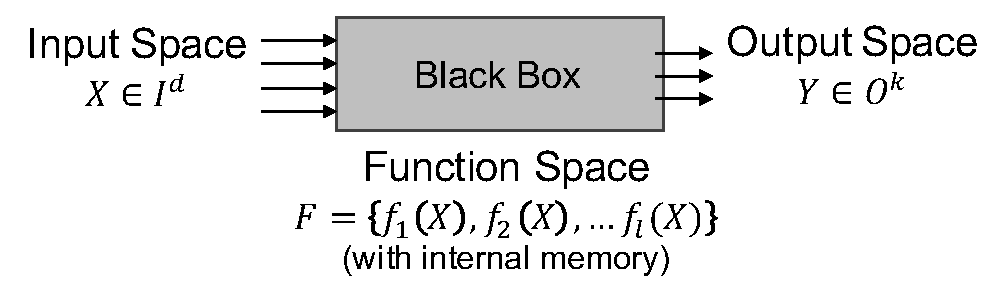
\includegraphics[width=0.9\columnwidth]{figures/blackbox_model.pdf}
    \vspace*{-4mm}
    \caption{Example figure}
    \label{fig:example_figure}
\end{figure}
			\section{Tables} \label{sec:examples_tables}
Tables should automatically be adjusted by the template. Table~\ref{table:table_format} shows the important rules and Table~\ref{table:example_table} provides an example.

%Table: Table format
\begin{table}[H]
    \centering
\begin{threeparttable}[H]
    \renewcommand{\arraystretch}{1.3}
    \caption{Figure format}
    \label{table:table_format}
    \setlength\tabcolsep{5pt}
    \begin{tabular}{|l|l|l|}\hline
        \tableheader Item &\tableheader LUH &\tableheader SPbPU \\\hline

        Title Font        &Normal      &Italic\\\hline
        Title Location    &Above       &Above\\\hline
        Title Alignment   &Centered    &Left\\\hline
        Number            &7.3         &7.3\\\hline
        Seperator         &:           &-\\\hline

    \end{tabular}
\end{threeparttable}
\end{table}

%Table: Example instances of knowledge with descriptions
\begin{table}[H]
    \centering
\begin{threeparttable}[H]
    \renewcommand{\arraystretch}{1.3}
    \caption{Example instances of knowledge with descriptions}
    \label{table:example_table}
    \setlength\tabcolsep{5pt}
    \begin{tabular}{|l|l|l|}\hline
        \tableheader Instance
        &\tableheader Knowledge Content
        &\tableheader Description
        \\\hline

        $c_1$       &($x_1=0.0$)        &Input $x_1$ has a value 0.0. \\\hline
        $c_2$       &($x_1=1.0$)        &Input $x_1$ has a value 1.0. \\\hline
        $c_3$       &($x_2=0.0$)        &Input $x_2$ has a value 0.0. \\\hline
        $c_4$       &($x_2=1.0$)        &Input $x_2$ has a value 1.0. \\\hline
        $c_5$       &($y_1=0.0$)        &Output $y_1$ has a value 0.0 \\\hline
        $c_6$       &($y_1=1.0$)        &Output $y_1$ has a value 1.0 \\\hline
        $c_7$       &($c_1$, $c_3$)     &$x_1=0$ and $x_2$=0 simultaneously. \\\hline
        $c_8$       &($c_1$, $c_4$)     &$x_1=0$ and $x_2$=1 simultaneously. \\\hline
        $c_9$       &($c_2$, $c_3$)     &$x_1=1$ and $x_2$=0 simultaneously. \\\hline
        $c_{10}$    &($c_2$, $c_4$)     &$x_1=1$ and $x_2$=1 simultaneously. \\\hline
        $c_{15}$    &($c_{14}$; $3c_2$; $c_{13}$)   &\makecell[l]{$x_1$ switched from 0 to 1, held for 3$t$\\ then switched to 0.}\\\hline
    \end{tabular}
\end{threeparttable}
\end{table}
			\section{Equations} \label{sec:examples_equations}
Equations are partly automatic. The number scheme is automatic, but the commas and period must be manually added/removed for the two versions. Table~\ref{table:equations_format} shows the important rules and the below equations provide an example.

%Table: Table format
\begin{table}[H]
    \centering
\begin{threeparttable}[H]
    \renewcommand{\arraystretch}{1.3}
    \caption{Figure format}
    \label{table:equations_format}
    \setlength\tabcolsep{5pt}
    \begin{tabular}{|l|l|l|}\hline
        \tableheader Item &\tableheader LUH &\tableheader SPBPU \\\hline

        Suffix            &None        &commas ending with period\\\hline
        Eq. Location      &Centered    &Centered\\\hline
        Number Location   &Right       &Right\\\hline
        Number Style      &(7.3)       &(7-3)\\\hline

    \end{tabular}
\end{threeparttable}
\end{table}

\begin{align}
    \label{eqn:bin_count}
    N       &= \sum 1_t \\
    \label{eqn:bin_sum}
    Sum     &= \sum v_t \\
    \label{eqn:bin_sqsum}
    SqSum   &= \sum {v_t}^2 \\
    \label{eqn:bin_avg}
    \avg    &= Sum/N \\
    \label{eqn:bin_stddev}
    \stddev  &= SqSum - 2N\avg + N\avg^2
\end{align}

\begin{align}
    \label{eqn:bin_count2}
    N       &= \sum 1_t, \\
    \label{eqn:bin_sum2}
    Sum     &= \sum v_t, \\
    \label{eqn:bin_sqsum2}
    SqSum   &= \sum {v_t}^2, \\
    \label{eqn:bin_avg2}
    \avg    &= Sum/N, \\
    \label{eqn:bin_stddev2}
    \stddev  &= SqSum - 2N\avg + N\avg^2.
\end{align} \clearpage
			\section{Algorithms} \label{sec:examples_algorithms}
Algorithms are not automatic. LUH prefers the algorithmic style while SPbPU requires figures. Below are examples of both.

Note: The caption of the below figure has been overridden to follow the SPbPU format. 

Warning: This changes the list of figures/algorithms as well as the counts. 

%Alg: Split range
\begin{algorithm}[H]
    \centering
    \footnotesize
    %\scriptsize
    \begin{algorithmic}[1]
        \LineComment{Global variable}
        \State $R \gets rangesList$
        \Procedure{SplitRange}{$r, value$}
            \LineComment{Create new ranges}
            \State $rLow \gets range(r.Low, value)$
            \State $rHigh \gets range(value, r.High)$
            
            \LineComment{Remove old range and add new ranges}
            \State $R.Remove(r)$
            \State $R.Add(rLow)$
            \State $R.Add(rHigh)$
        \EndProcedure
    \end{algorithmic}
    \caption{LUH Algorithm Example}
    \label{alg:luh_algorithm_example}
\end{algorithm}

%Alg: Split range
\begin{figure}[H]
    \centering
    \footnotesize
    %\scriptsize
    \fbox{\parbox{0.5\textwidth}{
        \begin{algorithmic}[1]
            \LineComment{Global variable}
            \State $R \gets rangesList$
            \Procedure{SplitRange}{$r, value$}
                \LineComment{Create new ranges}
                \State $rLow \gets range(r.Low, value)$
                \State $rHigh \gets range(value, r.High)$
                
                \LineComment{Remove old range and add new ranges}
                \State $R.Remove(r)$
                \State $R.Add(rLow)$
                \State $R.Add(rHigh)$
            \EndProcedure
        \end{algorithmic}
    }}
    %\caption{SPbPU algorithm example.}    
    %\label{fig:spbpu_algorithm_example}

    %Don't use the below caption line! This is only to show the example. Use the above caption and label lines.
    \caption*{\textit{Figure X.X - SPbPU Algorithm Example}} 
\end{figure}
		\chapter{Thesis Main Content} \label{chap:thesis_main_content}
Below are example sections for defining the main content. They are not necessarily required.
			\section{Part 1}
				\subsection{Content Subsection}
				\subsection{Content Subsection}
			\section{Part 2}
				\subsection{Content Subsection}
				\subsection{Content Subsection}
		\chapter{Experiments Setup} \label{chap:experiments_setup}
Below are example sections for defining the experimental setup. They are not necessarily required.
			\section{Datasets}
				\subsection{Datasets Subsection}
				\subsection{Datasets Subsection}
			\section{Equipment}
				\subsection{Equipment Subsection}
				\subsection{Equipment Subsection}
			\section{Processes}
				\subsection{Processes Subsection}
				\subsection{Processes Subsection}
		\chapter{Results} \label{chap:experiments_results}
Below are example sections for defining the experimental results. They are not necessarily required.
			\section{Results Section}
				\subsection{Results Subsection}
				\subsection{results Subsection}
			\section{Results Section}
				\subsection{Results Subsection}
				\subsection{results Subsection}	
		\chapter{Future Considerations} \label{chap:future_considerations}
			\section{Topic Points} \label{sec:topic_points}
It is very likely that the new thesis will solve all problems and have no room for development or improvements. As such, these ideas should be documented and briefly introduced here to encourage others to build upon the new work described in the thesis. The formatting here is only for example.

Below is a list of topics that became apparent during development and testing of this work. They are not meant to be extensive, but rather to provide insight about any future developments. Entries in \textbf{bold} have proposed extensions in section~\ref{sec:proposed_extensions}.

\begin{enumerate}
    \item \textbf{Algorithms} – SPBPU requires algorithms to be figures and generally other scientific writers prefer the algorithmic format. This is not part of the automatic formatting.
    \item \textbf{Equations} – SPBPU requires equations to be the end of a sentence and be seperated by commas. LUH does not have this requirement. This is not part of the automatic formatting.
\end{enumerate}
 \clearpage
			\section{Proposed Extensions} \label{sec:proposed_extensions}
\begin{enumerate}
    \item \textbf{Algorithms} - SPbPU requires algorithms to be displayed as figures. Normally algorithms are displayed via the algorithm enviornment. A new environment could be created for changing the location of the figure name and number automatically as well as placing the content in a box.
    
    \item \textbf{Equations} - SPbPU requires equations to be formatted as the end of a sentance with commas and a period. A new enviornment could be created with an option to turn these commas and period on/off. This would enable all this format to be adjust from the template, rather than in the content itself.
\end{enumerate}


		\chapter{Conclusions} \label{chap:conclusions}
An adaptive template has been created for semi-automating the formatting of a master thesis. This LaTeX template serves to create two versions, one for Leibniz University Hannover and one for Peter the Great Saint Petersburg Polytechnic University.

A main.tex file is created for both universities, which defines the standard formatting rules for each university and then references various content files with minimal formatting. When compiled two seperated documents are produced from the same content.

To support further development, this work is available at \url{ https://github.com/chriswblake/ThesisTemplate_LUH_SPBSTU}
	
	\appendix
		\chapter{Title of A}
			\section{Abreviations} % Optional, if needed.
			\section{Software Used} % Optional, if needed
			\section{Figures} % Optional, if needed
		\chapter{Title of B}
			\section {Code 1}
			\section {Code 2}

	\backmatter
		\bibliographystyle{plain}
		\bibliography{references}

	\end{document}